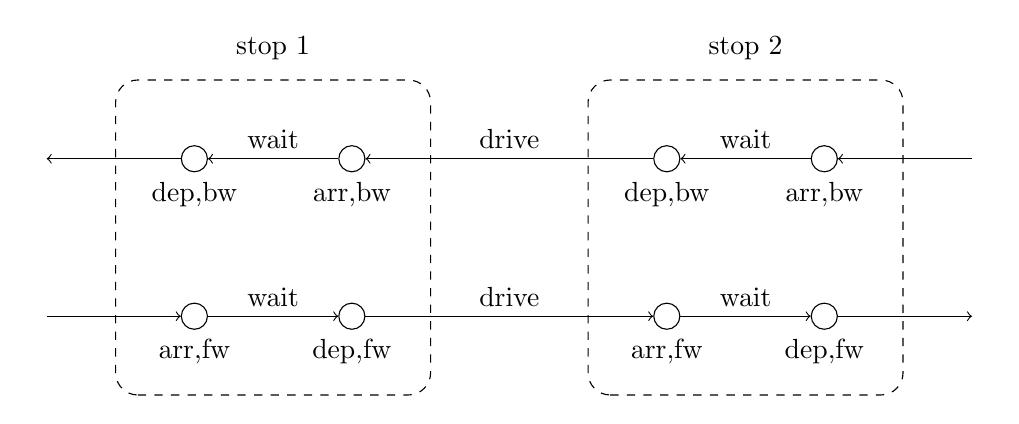
\begin{tikzpicture}[scale=2]
% \node {Hei moi!};
\tikzstyle{node}=[circle,draw]


% \foreach \x in {0,1}
%     \foreach \y in {0,1}
%         \node (s1-\x-\y) at (\x, \y) [node,label=] {};
% \foreach \y in {0, 1}
%     \node (s1-ext-\y) at (-1, \y) {};

\node (0-0) at (0, 0) [node, label={below:arr,fw}]{};
\node (1-0) at (1, 0) [node, label={below:dep,fw}]{};
\node (3-0) at (3, 0) [node, label={below:arr,fw}]{};
\node (4-0) at (4, 0) [node, label={below:dep,fw}]{};
\node (ext1-0) at (-1, 0) {};
\node (ext2-0) at (5, 0) {};


\node (0-1) at (0, 1) [node, label={below:dep,bw}]{};
\node (1-1) at (1, 1) [node, label={below:arr,bw}]{};
\node (3-1) at (3, 1) [node, label={below:dep,bw}]{};
\node (4-1) at (4, 1) [node, label={below:arr,bw}]{};
\node (ext1-1) at (-1, 1) {};
\node (ext2-1) at (5, 1) {};


% \foreach \x in {3,4}
%     \foreach \y in {0,1}
%         \node (s2-\x-\y) at (\x, \y) [node] {};
% \foreach \y in {0, 1}
%     \node (s2-ext-\y) at (5, \y) {};

\draw [->] (ext1-0) to (0-0);
\draw [->] (0-0) to node [above] {wait} (1-0);
\draw [->] (1-0) to node [above] {drive} (3-0);
\draw [->] (3-0) to node [above] {wait} (4-0);
\draw [->] (4-0) to (ext2-0);

% Reverse direction for top row
\draw [->] (ext2-1) to (4-1);
\draw [->] (4-1) to node [above] {wait} (3-1);
\draw [->] (3-1) to node [above] {drive} (1-1);
\draw [->] (1-1) to node [above] {wait} (0-1);
\draw [->] (0-1) to (ext1-1);

\draw [rounded corners=8, dashed] (-0.5, -0.5) -- (1.5, -0.5)
    -- (1.5, 1.5) -- (-0.5, 1.5) -- cycle;

\draw [rounded corners=8, dashed, xshift=3cm] (-0.5, -0.5) -- (1.5, -0.5)
    -- (1.5, 1.5) -- (-0.5, 1.5) -- cycle;


\node at (0.5, 1.7) {stop 1};
\node at (3.5, 1.7) {stop 2};

\end{tikzpicture}